\documentclass{article}
\usepackage{amsmath, fullpage, listings, xcolor}
\usepackage{booktabs}
\usepackage{array}
\usepackage{graphicx}

% SQL syntax highlighting
\lstdefinestyle{sql}{
    language=SQL,
    basicstyle=\ttfamily\footnotesize,
    keywordstyle=\color{blue}\bfseries,
    stringstyle=\color{red},
    commentstyle=\color{green},
    showstringspaces=false,
    breaklines=true,
    frame=single,
    backgroundcolor=\color{gray!10}
}

\lstset{style=sql}

\begin{document}
\title{Project 1: SQL Query Notes}
\author{Edward Song}
\maketitle
\thispagestyle{empty}

\section{Relational Algebra}

\subsection{Projection $(\pi)$}
All of the operators in relational algebra take a relation (table) as input and produce a relation as output. A basic query looks like this:

\[
\pi_{name}(dogs)
\]

The subscript of the $\pi$ operator specifies which columns to select. In this case, the operator takes the \texttt{dogs} relation in as a parameter and returns a relation that only has the \texttt{name} column of \texttt{dogs}.

The relational algebra expression above can be written in SQL as:
\begin{lstlisting}
SELECT name FROM dogs;
\end{lstlisting}

If the dogs relation is initially:

\begin{center}
\begin{tabular}{|c|c|}
\hline
\textbf{name} & \textbf{age} \\
\hline
Scooby & 10 \\
Buster & 15 \\
Buster & 20 \\
\hline
\end{tabular}
\end{center}

The query above would return:
\begin{center}
\begin{tabular}{|c|}
\hline
\textbf{name} \\
\hline
Scooby \\
Buster \\
\hline
\end{tabular}
\end{center}

\subsection{Selection $\sigma$}
The selection operator takes in a single relation and filters based on a certain condition. This operator is equivalent to the \texttt{WHERE} clause.

The query:
\begin{lstlisting}
    SELECT name, age FROM dogs WHERE age = 12;
\end{lstlisting}

can be expressed as
\[
\sigma_{age=12}(\pi_{name, age}(dogs)).
\]

Another correct expression for the query is:
\[
\pi_{name, age}(\sigma_{age=12}(dogs)).
\]

The selection operator can compound predicates. The $\wedge$ symbol corresponds to the AND keyword in SQL, and the $\vee$ symbol corresponds to the OR keyword.

For example,
\begin{lstlisting}
    SELECT name, age FROM dogs WHERE age = 12 AND name = 'Timmy';
\end{lstlisting}

is equivalent to

\[
\pi_{name, age}(\sigma_{age = 12 \wedge name = 'Timmy"}(dogs))
\]

\subsection{Union $(\cup)$}
\label{sec:Union}
Just like UNION in SQL, we take all the rows from each tuple and combine them removing duplicates along the way.

As an example, say we have a dogs table:

\begin{center}
\begin{tabular}{|c|c|}
\hline
\textbf{name} & \textbf{age} \\
\hline
Scooby & 10 \\
Buster & 15 \\
Garfield & 20 \\
\hline
\end{tabular}
\end{center}

and a cats table:

\begin{center}
\begin{tabular}{|c|c|}
\hline
\textbf{name} & \textbf{age} \\
\hline
Tom & 8 \\
Garfield & 10 \\
\hline
\end{tabular}
\end{center}

The expression:

\[
    \pi_{name}(dogs) \cup \pi_{name}(cats)
\]

would return:
\begin{center}
\begin{tabular}{|c|}
\hline
\textbf{name}\\
\hline
Scooby \\
Buster \\
Tom \\
Garfield \\
\hline
\end{tabular}
\end{center}

Garfield only shows up once because relations are sets of tuples and remove all duplicates as a result.

\subsection{Set Difference $(-)$}
Another set operator is the set difference operator. It returns every row in the first table except the rows that also show up in the second table. Set difference is equivalent to the SQL clause \texttt{EXCEPT}. If you run:
\[
\pi_{name}(dogs) - \pi_{name}(cats)
\]
expression on the dogs and cats table introduced in the previous section you would get:
\begin{center}
\begin{tabular}{|c|}
\hline
\textbf{name}\\
\hline
Scooby \\
Buster \\
\hline
\end{tabular}
\end{center}

Garfield does not show up because he is in the cats table, and none of the cats’ names will show up because it is only possible for rows from the first relation to show up in the output.

\subsection{Intersection $(\cap)$}
Intersection is just like the \texttt{INTERSECT} SQL operator in that it only keeps rows that occur in both tables. If you run:

\[
\pi_{name}(dogs) \cap \pi_{name}(cats)
\]

on the table from subsection~\ref{sec:Union}, you would get:

\begin{center}
\begin{tabular}{|c|}
\hline
\textbf{name}\\
\hline
Garfield \\
\hline
\end{tabular}
\end{center}

because Garfield is the only name to occur in both tables.

\subsection{Cross Product $(\times)$}
The cross product operator is just like performing a Cartesian product in SQL. The output is one tuple for every possible pair of tuples from both relations. As an example, say we have a dogs table:

\begin{center}
\begin{tabular}{|c|c|}
\hline
\textbf{name} & \textbf{age} \\
\hline
Scooby & 10 \\
Buster & 15 \\
Garfield & 20 \\
\hline
\end{tabular}
\end{center}

and a parks table:

\begin{center}
\begin{tabular}{|c|c|}
\hline
\textbf{park} & \textbf{city} \\
\hline
Golden Gate Park & San Francisco \\
Central Park & New York City \\
\hline
\end{tabular}
\end{center}

The relational algebra equivalent of

\begin{lstlisting}
    SELECT * FROM dogs, parks;
\end{lstlisting}
is
\[
    dogs \times parks
\]

and the output will be:

\begin{center}
\begin{tabular}{|c|c|c|c|}
\hline
\textbf{name} & \textbf{age} & \textbf{park} & \textbf{city} \\
\hline
Scooby & 10 & Golden Gate Park & San Francisco \\
Scooby & 10 & Central Park & New York City \\
Buster & 15 & Golden Gate Park & San Francisco \\
Buster & 15 & Central Park & New York City \\
Garfield & 20 & Golden Gate Park & San Francisco \\
Garfield & 20 & Central Park & New York City \\
\hline
\end{tabular}
\end{center}

\subsection{Joins $(\bowtie)$}
To inner join two tables, write the left table on the $\bowtie$ operator, put the join condition in the subscript, and put the right operator on the right side. To join together the cats table with the dogs table on the name column, you would write:
\[
cats\bowtie_{cats.name = dogs.name} dogs
\]

The $\bowtie$ operator performs an inner join, which is the only join we will cover for relational algebra expressions in this class.

The join operator $\bowtie$ also supports the compound predicate operators $\wedge$ (AND) and $\vee$ (OR).


\subsection{Rename $(\rho)$}
The rename operator is used to change the name of a specified column. For instance, to rename the \textit{dogs} relation’s \textit{name} column to \textit{dname}, we can write:
\[
\textit{cats} \bowtie_{name = dname} \rho_{name \rightarrow dname}(\textit{dogs}).
\]

\subsection{Group By / Aggregation $(\gamma)$
}

The group by / aggregation operator is equivalent to using \texttt{GROUP BY} and \texttt{HAVING} in SQL. For example, the SQL query

\begin{lstlisting}
    SELECT age FROM dogs GROUP BY age HAVING COUNT(*) > 5;
\end{lstlisting}

can be expressed in relational algebra as

\[
    \gamma_{age, COUNT(*)>5}(dogs).
\]

\subsection{Practice Questions}

Given the following two relations:
\begin{lstlisting}
teams(teamid, name)
\end{lstlisting}

\begin{lstlisting}
players(playersid, name, teamid, position)
\end{lstlisting}

\textbf{1. Write an expression that finds the name and playerid of every player that plays the “center" position.
}
\[
\pi_{name, playerid}(\sigma_{position = 'center'}(players))
\]
We first filter out the rows for players who aren’t centers, then we project only the columns that we need.

\textbf{2. Write an expression that finds the name of every player that plays on the "Warriors".}

\[
    \pi_{players.name}(\sigma_{teams.name = 'Warriors'}(players \bowtie_{players.teamid = teams.teamid} teams)))
\]

We first join together the teams and players table to get all the information we need. Then we filter out the rows that aren't players who play for the warriors. Lastly, we project only the column that we're looking for.

\textbf{3. Write an expression that finds the teamid of all teams that do not have any players.}

\[
\pi_{teamid}(teams) - \pi_{teamid}(players)
\]

All teams must be in the teams table, so we first get all of their teamids. Then we subtract all teamids that appear in players, because if that teamid appears in players, the team has players. We are then left with only teamids of teams that don't have any players.

\textbf{4. Write an expression that is equivalent to the following SQL query:}

\begin{lstlisting}
SELECT teamid AS tid 
FROM players
WHERE players.teamid NOT IN
    (SELECT teamid FROM teams)
AND position='shooting guard'
\end{lstlisting}

We want shooting guards that aren't on a team.

\[
\rho_{teamid \rightarrow tid}(\pi_{teamid}(\sigma_{position = 'shooting \text{ } guard'}(players)) - \pi_{teamid}(teams))
\]

We first filter out rows for players who aren’t shooting guards, then we only project the column we need, teamid. We then use set difference to only keep players who play for a team not in the teams table. Finally, we use the renaming operator to rename teamid to tid.


\section{Hashing}
\subsection{Motivation}
Sometimes we want to group the same value together, but we don't actually care about order. 

\subsection{General Strategy}
In a database, we can't fit all data in RAM at once, so we need to build several hash tables build hash tables and combine them. There is a problem with this idea though. What happens if we build two separate hash tables that each have the same value in them (e.g. “Brian” occurs in both tables)? Combining the the tables will result in some of the “Brian”s not being right next to each other.

To fix this, before building a hash table out of data in memory, we need to guarantee that if a certain value is in memory, all of its occurrences are also in memory. So if "Brian" occurs in memory at least once, then we can only build the hash table if every occurrence of “Brian” in our data is currently in memory. This ensures that values can only appear in one hash table, making the hash tables safe to concatenate.

\subsection{The Algorithm}
In the following example, we will assume that we have $B = 3$ buffer pages available to us. We also assume that Brian and Eric hash to the same value for the first hash function but different values for the second hash function, and Jamie and Lakshya hash to the same value for the first hash function.

\begin{figure}[h]
    \centering
    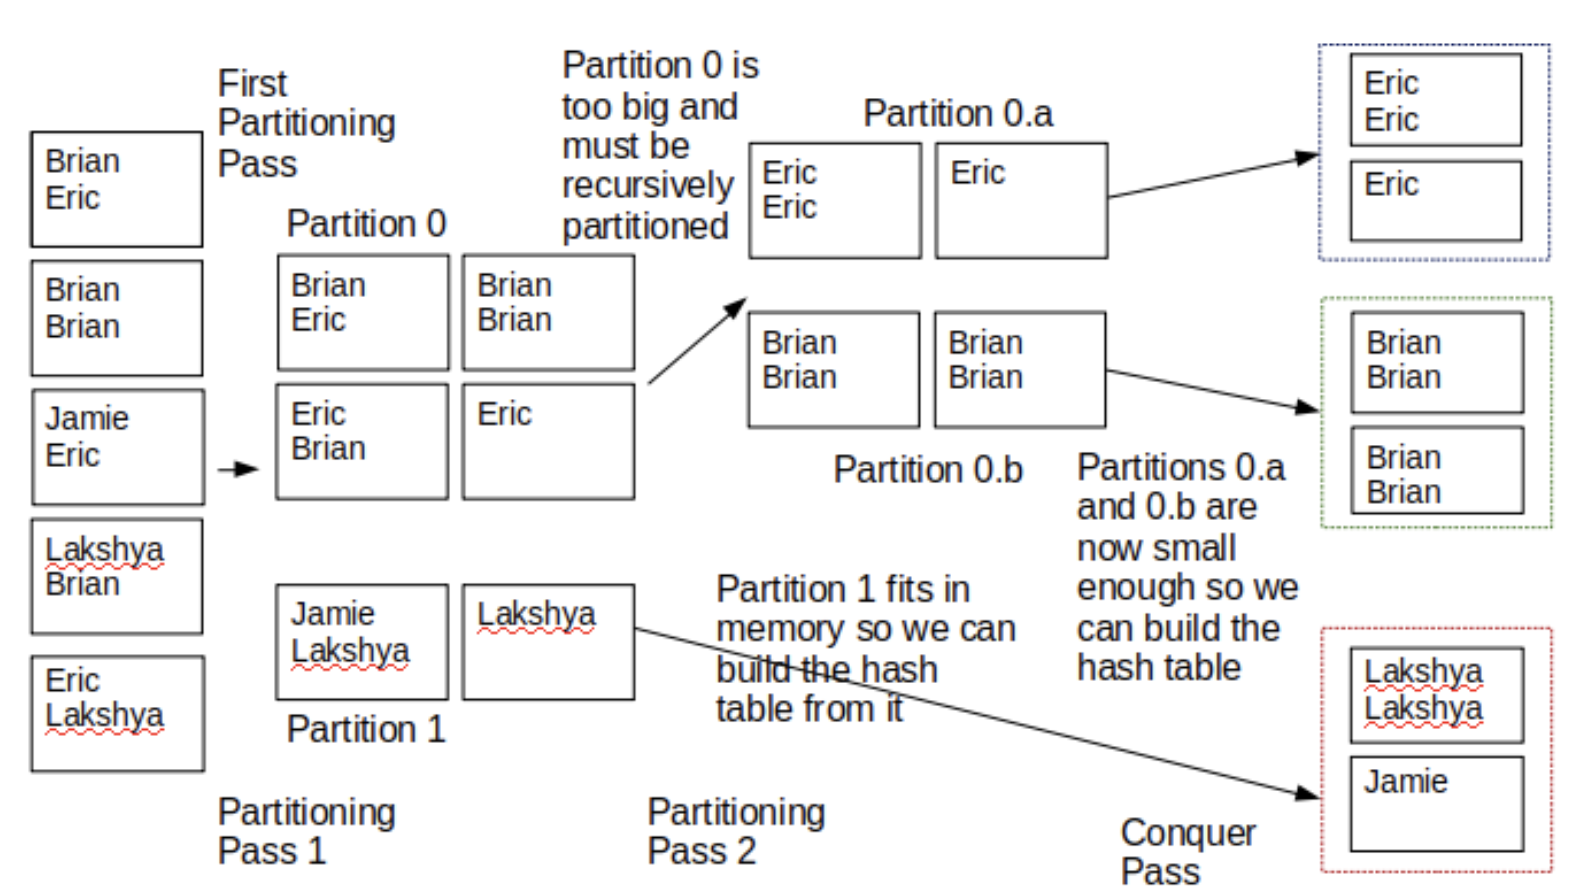
\includegraphics[width=0.8\linewidth]{images/Hashing.png}
    \caption{After the first partitioning pass (Partitioning Pass 1), Partition 0 is 4 pages, and Partition 1 is 2 pages. Partition 1 fits in memory, but Partition 0 does not. This means we must recursively partition 0.}
    \label{fig:placeholder}
\end{figure}

1. After Partitioning Pass 2, Partition 0 is broken into two parts: Partition 0.a is 2 pages, and Partition 0.b is 2 pages. As Partition 1 already fit into memory, it was not partitioned during Partitioning Pass

2. Once all partitions (0.a, 0.b, 1) fit into memory, we perform the Conquer Pass and build the hash tables. You can see that after the final Conquer Pass, all of the like values are next to each other, which is our end goal.


\end{document}
